\addtocontents{toc}{\protect\setcounter{tocdepth}{0}} 

\chapter{Příklady použití a testování časové náročnosti} 

  \paragraph{ } Vyzkoušíme nyní algoritmus na několika příkladech. Poté provedeme srovnání 
  času potřebného pro výpočet s algoritmem $AlmostSplitSequence$ implementovaným v \cite{QPA}.
  Náš algoritmus pojmenujeme jednoduše $AlmostSplitSequence2$. 
  
  Pro testování 
  času necháme každý algoritmus provést výpočet několikrát následujícím 
  skriptem, kde ve funkci $GetModule$ znovu vytvoříme modul pro který počítáme. 
  Modul, jeho algebru i quiver je 
  třeba vždy vytvořit znova, aby GAP nemohl jeho generátor skoro štěpitelných 
  posloupností a další vlastnosti, které mohou zkreslit konečný čas, cacheovat (neboli pamatovat si předchozí 
  výpočty pro urychlení budoucích operací).
  \begin{Verbatim}[frame=single,numbers=left]
GetModule := function(i)
  local K, Q, KQ, A, matrices, mX;

  K := Rationals;
  Q := Quiver(3, [[1, 2, "a"], [2, 3, "b"],[1, 3, "c"]]);
  A := PathAlgebra(K,Q);
  matrices := [ ["a", [[1,0,0],[0,1,0]]], 
                ["b", [[0,1],[1,0],[0,1]]], 
                ["c", [[0,0],[1,0]]] ];
  mX := RightModuleOverPathAlgebra(A,matrices);

  return mX;
end;

TestPerformance := function(iter)
  local i, time;

  time := Runtime();
  for i in [1..iter] do
    AlmostSplitSequence( GetModule(i) );
  od;
  time := Float((Runtime() - time) / iter / 1000);
  Print("Execution time for AlmostSplitSequence: ", time, "\n");

  time := Runtime();
  for i in [1..iter] do
    AlmostSplitSequence2( GetModule(i) );
  od;
  time := Float((Runtime() - time) / iter / 1000);
  Print("Execution time for AlmostSplitSequence2: ", time, "\n");
end;

TestPerformance(100);
  \end{Verbatim} 
  
      \subsection*{Příklad 1}
        \paragraph{ } Nechť $K$ je těleso racionálních čísel a toulec $Q$, přípustný ideál $I$ a $A$-modul $X$, 
        kde algebra $A=KQ/I$, jsou dány následovně: \\\\
        \centerline{
          Toulec $Q$: \xymatrix{
            \circ^1 \ar@{->}[r]_a \ar@/^3pc/[rr]^c
              & \circ^2 \ar@{->}[r]_b
              & \circ^3
          }
          \rightaligned{
            \space\space\space\space $I=\emptyset$ \space\space\space\space
             A-modul $X$: \xymatrix{
               K^2 
                   \ar@{->}[r]_{\left[\begin{smallmatrix}
	               1 & 0 \\
	               0 & 1 \\
                      \end{smallmatrix}\right]} 
                   \ar@/^3pc/[rr]^{\left[\begin{smallmatrix}
	               1 \\
	               0 \\
                      \end{smallmatrix}\right]}
                 & K^2 
                   \ar@{->}[r]_{\left[\begin{smallmatrix}
	               0 \\
	               1 \\
                      \end{smallmatrix}\right]}   
                 & K^1
             }
           }
         }\\\\\\
         Výsledný generátor množiny skoro štěpitelných posloupností je: 
         \\\\
         \centerline{\xymatrix{
            DTr(X) \ar@{->}[ddddd]
                 & 
                 & K^4
                   \ar@{.>}[ddddd]_{\left[\begin{smallmatrix}
	               1 & 0 & 0 & 0 & 0 & 0\\
	               0 & 1 & 0 & 0 & 0 & 0\\
	               0 & 0 & 1 & 0 & 0 & 0 \\       
	               0 & 0 & 0 & 1 & 0 & 0 \\       
	               \end{smallmatrix}\right]}
                   \ar@{->}[r]_{\left[\begin{smallmatrix}
	               0 & 0 & 0\\
	               1 & 0 & 0\\
	               0 & 0 & 1\\   
	               0 & 1 & 0 \\    
                      \end{smallmatrix}\right]} 
                   \ar@/^3pc/[rr]^{\left[\begin{smallmatrix}
	               1 & 0 & 0 \\
	               0 & 0 & -1 \\
	               0 & 1 & 0 \\
	               0 & 0 & 0 \\
                      \end{smallmatrix}\right]}
                 & K^3
                   \ar@{.>}[ddddd]|-{\left[\begin{smallmatrix}
	               1 & 0 & 0 & 0 & 0\\
	               0 & 1 & 0 & 0 & 0\\
	               0 & 0 & 1 & 0 & 0\\       
	               \end{smallmatrix}\right]}
                   \ar@{->}[r]_{\left[\begin{smallmatrix}
	               1 & 0 & 0 \\
	               0 & 1 & 0 \\
	               0 & 0 & 1 \\
                      \end{smallmatrix}\right]}   
                 & K^3
                   \ar@{.>}[ddddd]^{\left[\begin{smallmatrix}
	               1 & 0 & 0 & 0\\
	               0 & 1 & 0 & 0\\
	               0 & 0 & 1 & 0\\              
	               \end{smallmatrix}\right]}
                 \\ \\ \\ \\ \\
            E  \ar@{->}[dddd]
                 & 
                 & K^6
                   \ar@{.>}[dddd]
                   \ar@{->}[r]_{\left[\begin{smallmatrix}
	               0 & 0 & 0 & 0 & 0\\
	               1 & 0 & 0 & 0 & 0\\
	               0 & 0 & 1 & 0 & 0\\
	               0 & 1 & 0 & 0 & 0\\
	               0 & 0 & 0 & 1 & 0\\
	               0 & 0 & 0 & 0 & 1\\                      
	               \end{smallmatrix}\right]} 
                   \ar@/^3pc/[rr]|-{\left[\begin{smallmatrix}
	               1 & 0 & 0 & 0 \\
	               0 & 0 & -1 & 0 \\
	               0 & 1 & 0 & 0 \\
	               0 & 0 & 0 & 0 \\
	               0 & 0 & 0 & 1 \\        
	               0 & 0 & 0 & 0 \\                   
	               \end{smallmatrix}\right]}
                 & K^5  
                   \ar@{.>}[dddd]
                   \ar@{->}[r]_{\left[\begin{smallmatrix}
	               1 & 0 & 0 & 0\\
	               0 & 1 & 0 & 0\\
	               0 & 0 & 1 & 0\\
	               1 & 0 & 0 & 0\\
	               0 & 0 & 0 & 1\\                      
                      \end{smallmatrix}\right]}   
                 & K^4
                   \ar@{.>}[dddd] 
                   \\ \\ \\ \\
            X
                 & 
                 & K^2 
                   \ar@{->}[r]_{\left[\begin{smallmatrix}
	               1 & 0 & 0 \\
	               0 & 1 & 0 \\
                      \end{smallmatrix}\right]} 
                   \ar@/_3pc/[rr]_{\left[\begin{smallmatrix}
	               0 & 0 \\
	               1 & 0 \\
                      \end{smallmatrix}\right]}
                 & K^3 
                   \ar@{->}[r]_{\left[\begin{smallmatrix}
	               0 & 1 \\
	               1 & 0 \\
	               0 & 1 \\
                      \end{smallmatrix}\right]}   
                 & K^2
         }} \\\\\\         
       \paragraph{ }Náš algoritmus byl v tomto poměrně jednoduchém případě pomalejší. Integrovaná 
       funkce $AlmostSplitSequence$ běžela v průměru ze 100 běhů 0,171s a naše 
       funkce $AlmostSplitSequence2$ průměrně 0.238s.
       
       \subsection*{Příklad 2}
        \paragraph{ }Otestujeme nyní algoritmus na mírně složitějším příkladě.
        Nechť $K$ je těleso racionálních čísel a toulec $Q$, přípustný ideál $I$ a $A$-modul $X$, kde algebra $A=KQ/I$, 
        jsou dány následovně: \\\\
        \centerline{
          $Q$: \xymatrix{
            \circ^1 
                \ar@/^1pc/[r]^a 
                \ar@/_1pc/[r]_b 
              & \circ^2 
                \ar@{->}[r]_d
                \ar@(lu,ru)[]^c
              & \circ^3
                \ar@/^3pc/[ll]^e
          }
          \rightaligned{
            \space\space\space\space $I=\{c^2,acd-bd,ea,eb\}$ \space\space\space\space
             $X$: \xymatrix{
            K^2 
                \ar@/^1pc/[r]^{\left[\begin{smallmatrix}
	               0 & 1 \\
	               1 & 1 \\
                      \end{smallmatrix}\right]} 
                \ar@/_1pc/[r]_{\left[\begin{smallmatrix}
	               1 & 0 \\
	               1 & 0 \\
                      \end{smallmatrix}\right]} 
              & K^2 
                \ar@{->}[r]_{\left[\begin{smallmatrix}
	               1 & 1 \\
	               0 & 1 \\
                      \end{smallmatrix}\right]}
                \ar@(lu,ru)[]^{\left[\begin{smallmatrix}
	               0 & 0 \\
	               1 & 0 \\
                      \end{smallmatrix}\right]}
              & K^2
                \ar@/^3pc/[ll]^{\left[\begin{smallmatrix}
	               0 & 0 \\
	               0 & 0 \\
                      \end{smallmatrix}\right]}             
             }
           }
         }\\\\
         Výsledný generátor množiny skoro štěpitelných posloupností je: 
         \\\\
         \centerline{\xymatrix{
            DTr(X) \ar@{->}[dd]
                & 
                & K^{10} 
                  \ar@/^1pc/[r]
                  \ar@/_1pc/[r]
                  \ar@{.>}[dd]
                & K^{6} 
                  \ar@{->}[r]
                  \ar@(lu,ru)[]
                  \ar@{.>}[dd]
                & K^{4}
                  \ar@/^3pc/[ll]   
                  \ar@{.>}[dd] 
                 \\ \\
            E  \ar@{->}[dd]
                & 
                & K^{12} 
                  \ar@/^1pc/[r]
                  \ar@/_1pc/[r]
                  \ar@{.>}[dd]
                & K^{8} 
                  \ar@{->}[r]                  
                  \ar@(lu,ru)[]
                  \ar@{.>}[dd]
                & K^{6}
                  \ar@/^3pc/[ll]   
                  \ar@{.>}[dd]
                 \\ \\
            X
                & 
                & K^2
                  \ar@/^1pc/[r]
                  \ar@/_1pc/[r]
                & K^2 
                  \ar@{->}[r]
                  \ar@(lu,ru)[]
                & K^2
                  \ar@/^3pc/[ll]   
         }} \\\\\\         \\\\
       \paragraph{ }Náš algoritmus již byl v tomto mírně složitějším případě rychlejší. Integrovaná 
       funkce $AlmostSplitSequence$ běžela v průměru ze 20 běhů 25s a naše 
       funkce $AlmostSplitSequence2$ průměrně 4s.
       \\\\
                      
       \subsection*{Příklad 3}
       
         \paragraph{ }        Nyní si ukážeme, jak je možné algoritmus 
         u algeber nad konečným tělesem, 
         které mají až na izomorfismus konečně mnoho nerozložitelných 
         reprezentací, využít k jejich výpočtu. Začneme s libovolným 
         neprojektivním a nerozložitelným modulem $X$. Spočteme jeho skoro 
         štepitelnou posloupnost \\\\
         \centerline{$0 \to DTr(X) \to E \to X \to 0$.} \\\\
         Poté modul $E$ rozložíme na nerozložitelné direktní sčítance a postup 
         opakujeme s každým z nich. Po konečném počtu kroků obdržíme 
         již pouze moduly izomorfní dříve nalezeným. Užitý postup nebudeme 
         dokazovat ani dopodrobna rozebírat, jde jen o základní ilustraci 
         využití zkonstruovaného algoritmu.
                  
         Nechť $K=GF(13)$ (Galois Field), $K$-algebra $A=KQ$, kde toulec $Q$ je dán následovně:\\\\
         \centerline{
         \xymatrix{
            & \circ^2  \\
            & \circ^1 \ar[rd] \ar[ld] \ar[u]\\
            \circ^3 & & \circ^4
          }}\\\\\\
          Začněme s neprojektivním jednoduchým nerozložitelným modulem $S(1)$:\\\\
         \centerline{
         \xymatrix{
           & 0  \\
            & K \ar[rd] \ar[ld] \ar[u] \\
            0 & & 0
          }}\\\\\\
          Ten i všechny ostatní moduly budeme pro jednoduchost zapisovat následovně s vynecháním šipek: \\\\
          \centerline{\begin{matrix}
               & 0       \\
               & 1 &    \\
            0 &    & 0   
          \end{matrix}} \\\\\\
          Máme jeho skoro štěpitelnou posloupnost\\\\
         \centerline{
         \xymatrix{
            DTr(X)={\begin{matrix} & 1 \\ & 2 & \\ 1 &  & 1\end{matrix}} \ar[rr]
            & & E_1= {\begin{matrix} & 1 \\ & 3 & \\ 1 &  & 1\end{matrix}} \ar[rr]
            & & S(0)={\begin{matrix} & 0 \\ & 1 & \\ 0 &  & 0\end{matrix}}
          },}\\\\\\
          kde $E_1$ rozložíme na 3 nerozložitelné direktní sčítance $N_1$, $N_2$, $N_3$ 
          a dostaneme diagram:\\\\
         \centerline{
         \xymatrix{
            & &  N_1={\begin{matrix} & 0 \\ & 1 & \\ 1 &  & 0\end{matrix}} \ar[rrd] \\
            DTr(X)={\begin{matrix} & 1 \\ & 2 & \\ 1 &  & 1\end{matrix}} \ar[rr] \ar[rru] \ar[rrd]
            & &  N_2={\begin{matrix} & 0 \\ & 1 & \\ 0 &  & 1\end{matrix}} \ar[rr]
            & & S(1)={\begin{matrix} & 0 \\ & 1 & \\ 0 &  & 0\end{matrix}} \\
            & &  N_3={\begin{matrix} & 1 \\ & 1 & \\ 0 &  & 0\end{matrix}} \ar[rru]
          }}\\\\\\
          Dále postup zopakujeme pro $DTr(X)$ a dostaneme diagram:\\\\
         \centerline{
         \xymatrix{
            & N_4={\begin{matrix} & 1 \\ & 1 & \\ 0 &  & 1\end{matrix}} \ar[rd]
              & &  {\begin{matrix} & 0 \\ & 1 & \\ 1 &  & 0\end{matrix}} \ar[rd] \\
            P(1)={\begin{matrix} & 1 \\ & 1 & \\ 1 &  & 1\end{matrix}} \ar[r] \ar[ru] \ar[rd]
              & N_5={\begin{matrix} & 1 \\ & 1 & \\ 1 &  & 0\end{matrix}} \ar[r]
              & {\begin{matrix} & 1 \\ & 2 & \\ 1 &  & 1\end{matrix}} \ar[r] \ar[ru] \ar[rd]
              & {\begin{matrix} & 0 \\ & 1 & \\ 0 &  & 1\end{matrix}} \ar[r]
              & {\begin{matrix} & 0 \\ & 1 & \\ 0 &  & 0\end{matrix}} \\
            & N_6={\begin{matrix} & 0 \\ & 1 & \\ 1 &  & 1\end{matrix}} \ar[ru]
              & &  {\begin{matrix} & 1 \\ & 1 & \\ 0 &  & 0\end{matrix}} \ar[ru]
          }}\\\\\\
          Pokud nyní spočteme skoro štěpitelné posloupnosti pro moduly $N_4$, 
          $N_5$ a $N_6$, tak všechny budou procházet projektivním modulem $P(1)$ 
          a začínat v jednom ze tří zbylých nerozložitelných projektivních 
          modulů. Tím jsme hotovi a náš diagram je kompletní:\\\\
         \centerline{
         \xymatrix{
            {\begin{matrix} & 0 \\ & 0 & \\ 1 &  & 0\end{matrix}} \ar[rd]
              & & {\begin{matrix} & 1 \\ & 1 & \\ 0 &  & 1\end{matrix}} \ar[rd]
              & &  {\begin{matrix} & 0 \\ & 1 & \\ 1 &  & 0\end{matrix}} \ar[rd] \\
            {\begin{matrix} & 0 \\ & 0 & \\ 0 &  & 1\end{matrix}} \ar[r]
              & {\begin{matrix} & 1 \\ & 1 & \\ 1 &  & 1\end{matrix}} \ar[r] \ar[ru] \ar[rd]
              & {\begin{matrix} & 1 \\ & 1 & \\ 1 &  & 0\end{matrix}} \ar[r]
              & {\begin{matrix} & 1 \\ & 2 & \\ 1 &  & 1\end{matrix}} \ar[r] \ar[ru] \ar[rd]
              & {\begin{matrix} & 0 \\ & 1 & \\ 0 &  & 1\end{matrix}} \ar[r]
              & {\begin{matrix} & 0 \\ & 1 & \\ 0 &  & 0\end{matrix}} \\
           {\begin{matrix} & 1 \\ & 0 & \\ 0 &  & 0\end{matrix}} \ar[ru]
              & & {\begin{matrix} & 0 \\ & 1 & \\ 1 &  & 1\end{matrix}} \ar[ru]
              & &  {\begin{matrix} & 1 \\ & 1 & \\ 0 &  & 0\end{matrix}} \ar[ru]
          }}\\\\\\
         Při našem pojmenování \\\\
         \centerline{
         \xymatrix{
            P(3) \ar[rd]
              & & N_4 \ar[rd]
              & & N_1 \ar[rd] \\
            P(4) \ar[r]
              &P(1) \ar[r] \ar[ru] \ar[rd]
              & N_5 \ar[r]
              & DTr(S(1)) \ar[r] \ar[ru] \ar[rd]
              & N_2 \ar[r]
              & S(1) \\
           P(2) \ar[ru]
              & & N_6 \ar[ru]
              & & N_3 \ar[ru]
          }}\\\\\\
          máme následující posloupnosti skoro štěpitelné posloupnosti \\\\
          \centerline{$   0\to P(3)\to P(1)\to N_4\to 0     $}
          \centerline{$   0\to P(4)\to P(1)\to N_5\to 0     $}
          \centerline{$   0\to P(2)\to P(1)\to N_6\to 0     $}
          \centerline{$   0\to N_4\to DTr(S(1))\to N_1\to 0     $}
          \centerline{$   0\to N_5\to DTr(S(1))\to N_2\to 0     $}
          \centerline{$   0\to N_6\to DTr(S(1))\to N_3\to 0     $}
          \centerline{$   0\to DTr(S(1))\to N_1\oplus N_2 \oplus N_3\to S(1)\to 0     $}
          \centerline{$   0\to P(1)\to N_4\oplus N_5\oplus N_6\to DTr(S(1)) \to 0     $}
          \\\\
          a navíc platí, že
          \begin{eqnarray}
            P(4) &=& S(4) \, = \, DTr(N_5)\nonumber \\
            P(3) &=& S(3) \, = \, DTr(N_6) \nonumber \\
            P(2) &=& S(2) \, = \, DTr(N_4) \nonumber \\
            P(0) &=& DTrDTr(S(1)) \nonumber \\
            N_4 &=& DTr(N_3) \nonumber \\
            N_5 &=& DTr(N_2) \nonumber \\
            N_6 &=& DTr(N_1). \nonumber
          \end{eqnarray}
          
          Měli jsme tedy více možností, jak při výpočtu postupovat a například 
          modul $N_6$ jsme mohli spočíst jako první modul skoro štěpitelné 
          posloupnosti končící v modulu $N_3$.
          
       \subsection*{Příklad 4}
       
         \paragraph{ } Zkusme nyní na srovnat rychlost obou algoritmů ve vztahu k počtu vrcholů a hran.
                   
          Nejprve budeme zvyšovat počet vrcholů a hran současně. 
          Opět položme $K=GF(13)$ (Galois Field) a $K$-algebru $A=KQ$, kde toulci $Q$ budeme 
          postupně navyšovat počet vrcholů od 2 do 20:\\\\
         \centerline{
         \xymatrix{
            \circ^2  \\
            \circ^1 \ar[u]
          }\\\\\\\\
         \xymatrix{
            \circ^2  \\
            \circ^1 \ar[d] \ar[u]\\
            \circ^3
          }\\\\
         \xymatrix{
            & \circ^2  \\
            & \circ^1 \ar[rd] \ar[ld] \ar[u]\\
            \circ^3 & & \circ^4
          }\\
         \xymatrix{
            \circ^2 & & \circ^3  \\
            & \circ^1 \ar[rd] \ar[ld] \ar[lu]  \ar[ru]\\
            \circ^ & & \circ^5
          }\\\\
         \xymatrix{
            \\
            \cdots
          }\\
          }\\\\
          
          Jako modul $X$, jehož skoro štěpitelnou posloupnost budeme hledat, zvolíme 
          neprojektivní, nerozložitelný a jednoduchý modul $S(1)$. Tedy modul, který 
          vrcholu $1$ přiřazuje vektorový prostor $K$, ostatním vrcholům nulový 
          vektorový prostor a šipkám nulová zobrazení.
          
          Nejprve se podíváme na rychlost v případě nízkého početu vrcholů toulce $Q$ a to $1,2,\ldots,7$:
        \\\\
\centerline{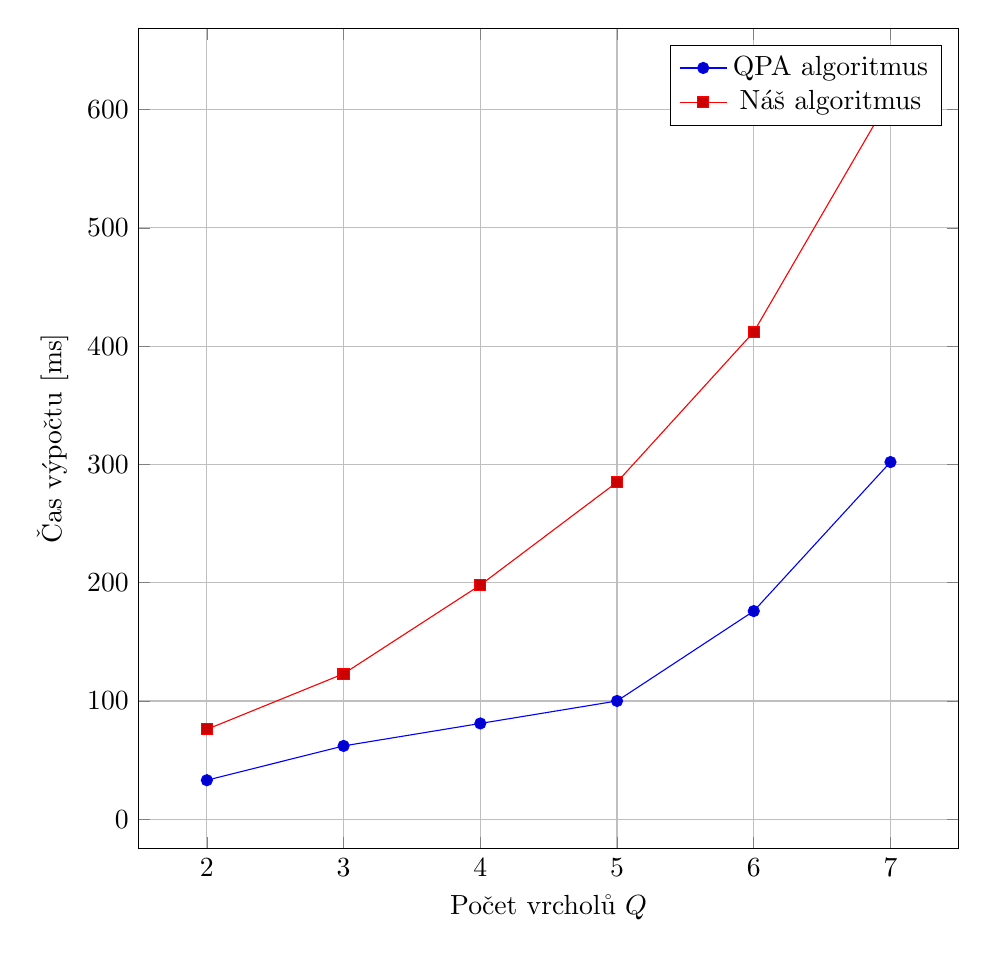
\begin{tikzpicture}
\begin{axis}[
xlabel={Počet vrcholů $Q$},
ylabel={Čas výpočtu [ms]},
grid=major, 
height=12cm,
width=12cm, ]
\addplot coordinates {
(2,33)
(3,62)
(4,81)
(5,100)
(6,176)
(7,302)
};
\addlegendentry{QPA algoritmus}
\addplot coordinates {
(2,76)
(3,123)
(4,198)
(5,285)
(6,412)
(7,611)
};
\addlegendentry{Náš algoritmus} 
\end{axis}
\end{tikzpicture}}
\paragraph{ }Jak vidíme, pro nízký počet vrcholů je náš algoritmus méně efektivní. Zhruba od 
velikosti toulce $|Q_0|=10$ ale začne původní algoritmus zaostávat  a to exponenciální 
rychlostí, jak je vidět na následujícím grafu:\\\\\\       
\centerline{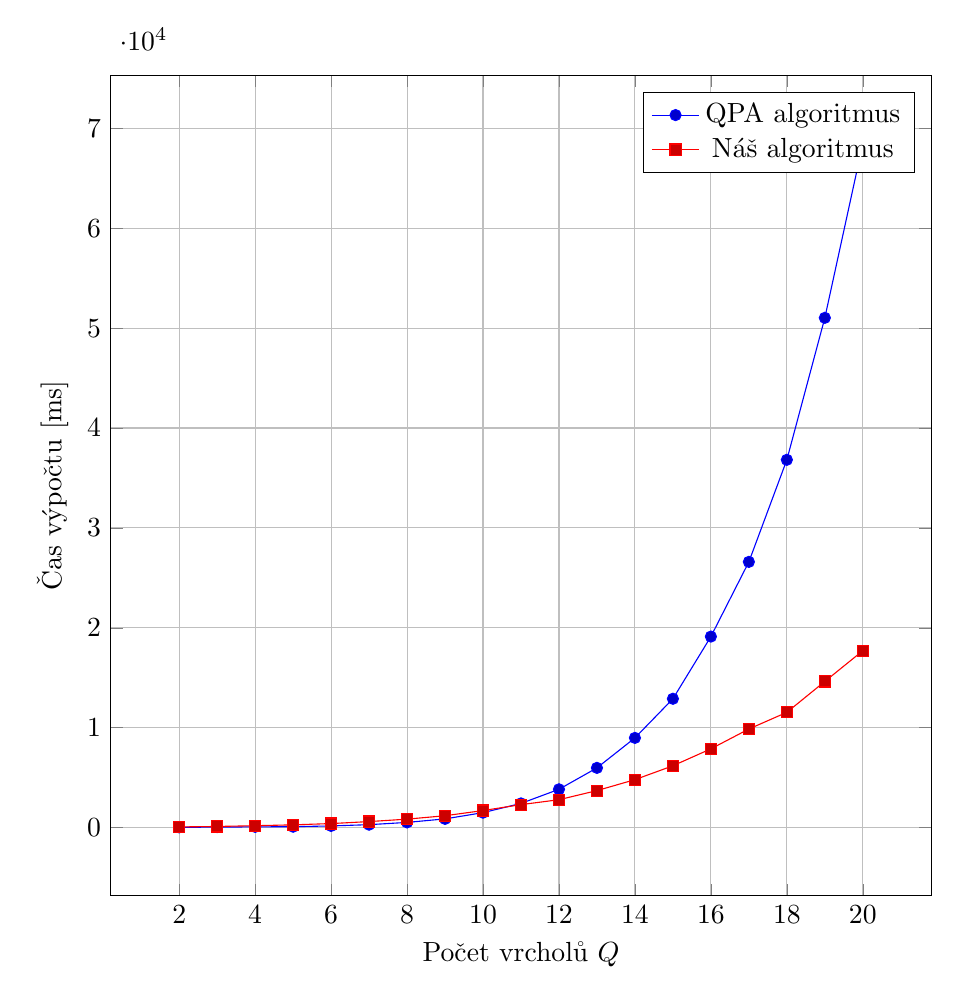
\begin{tikzpicture}
\begin{axis}[
xlabel={Počet vrcholů $Q$},
ylabel={Čas výpočtu [ms]},
grid=major, 
height=12cm,
width=12cm, ]
\addplot coordinates {
(2,33)
(3,62)
(4,81)
(5,100)
(6,176)
(7,302)
(8,528)
(9,881)
(10,1505)
(11,2429)
(12,3843)
(13,5986)
(14,8987)
(15,12902)
(16,19127)
(17,26604)
(18,36819)
(19,51028)
(20,68455)
};
\addlegendentry{QPA algoritmus}
\addplot coordinates {
(2,76)
(3,123)
(4,198)
(5,285)
(6,412)
(7,611)
(8,856)
(9,1196)
(10,1716)
(11,2307)
(12,2801)
(13,3712)
(14,4808)
(15,6196)
(16,7892)
(17,9877)
(18,11546)
(19,14637)
(20,17713)
};
\addlegendentry{Náš algoritmus} 
\end{axis}
\end{tikzpicture}}\\
    
Zkusme nyní zafixovat počet vrcholů na počtu 3 a zvyšovat počet hran. 
Toulec $Q$ budeme postupně ve 4 krocích konstruovat následovně:     \\\\
         \centerline{
         \xymatrix{
            \circ^2  \\
            \circ^1 \ar[d] \ar[u]\\
            \circ^3
          }\\\\
         \xymatrix{
            \circ^2  \\
            \circ^1 \ar@/^1pc/[d] \ar@/_1pc/[d]  \ar@/^1pc/[u] \ar@/_1pc/[u]\\
            \circ^3
          }\\\\
         \xymatrix{
            \circ^2  \\
            \circ^1 \ar[d] \ar@/^1pc/[d] \ar@/_1pc/[d] \ar[u] \ar@/^1pc/[u] \ar@/_1pc/[u]\\
            \circ^3
          }\\\\
         \xymatrix{
            \circ^2  \\
            \circ^1 \ar@/^1pc/[d] \ar@/_1pc/[d]  \ar@/^1pc/[u] \ar@/_1pc/[u] \ar@/^2pc/[d] \ar@/_2pc/[d]  \ar@/^2pc/[u] \ar@/_2pc/[u]\\
            \circ^3
          }
          }\\\\\\
    Jako modul $X$ opět jednoduše zvolíme modul $S(1)$. Z následujícího grafu je vidět ještě markatnější rozdíl
    v růstu výpočetního času mezi oběma algoritmy:
    \\\\\\       
\centerline{\begin{tikzpicture}
\begin{axis}[
xlabel={Počet hran vedoucích z vrcholu 1 do každého dalšího},
ylabel={Čas výpočtu [ms]},
grid=major, 
height=12cm,
width=12cm, ]
\addplot coordinates {
(1,52)
(2,253)
(3,4770)
(4,56743)q
};
\addlegendentry{QPA algoritmus}
\addplot coordinates {
(1,119)
(2,267)
(3,750)
(4,2505)
};
\addlegendentry{Náš algoritmus} 
\end{axis}
\end{tikzpicture}}\\
          
                 